\section{Inducción matemática}
\begin{itemize}
    \item El \emph{principio de inducción matemática} es una regla de inferencia utilizada para probar la verdad de proposiciones abiertas de una variable entera (se puede generalizar a no necesariamente enteros).
    \item La proposición abierta es una expresión que contiene una variable y que al ser sustituida dicha variable por un valor determinado, hace que la expresión se convierta en una proposición. 
    \item Sea $p(n)$ una proposición abierta definida sobre algún conjunto infinito de números enteros $S$.
        \begin{itemize}
            \item Es un conjunto infinito, nunca termina, se usa la inducción para conjuntos infinitos.
        \end{itemize}
        \[
          S = \{n_0,n_0+1,n_0+2,\dots\} 
        \]
    
    \item Utilizaremos la analogía del efecto \emph{dominó}, para representar cada parte del principio de inducción matemática.
    \item La proposición abierta es representada por una fila infinita de \emph{dominós}, cada uno de ellos asociados con exactamente elemento del conjunto $S$. 
    \item Si se cumplen las dos siguientes premisas/condición (premisas son proposiciones que se aceptan como verdaderas): 
        \begin{enumerate}
            \item $p(n_0)$ es verdadera.
                \begin{itemize}
                    \item Esto significa que el primer dominó caiga, el dominó puede caer.
                    \item Falso significa que no puede caer. 
                \end{itemize}

            \item Siempre que $p(k)$ es verdadera, entonces $p(k+1)$ también es verdadera, en donde $k \geq n_0$ .
                \begin{itemize}
                    \item En esta analogía, esto equivale a decir siempre que se cae el dominó asociado con $k$, entonces se cae el siguiente dominó asociado con $k+1$.
                \end{itemize}
            
            \item Entonces, la proposición $p(n)$ es verdadera para todo $n \in S$.
                \begin{itemize}
                    \item En la analogía esto equivale a decir que se caen todos los dominós.
                \end{itemize}
        \end{enumerate}
    
    \item En resumen el principio de inducción matemática establece que: 
        \begin{itemize}
            \item Dada una proposición abierta $p(n)$ definida $\forall n \in S = \{n_0,n_0+1,n_+2,\dots\}$. Si se cumple que: 
                \begin{enumerate}
                    \item $p(n_0)$ es verdadera, y 
                    \item $p(k) \implies p(k+1)$.
                \end{enumerate}
            
            \item Entonces la proposición $p(n)$ es verdadera $\forall n \in S$.
        \end{itemize}
\end{itemize}

\subsection{¿Para qué nos sirve la inducción?}
\begin{figure}[H]
    \centering
    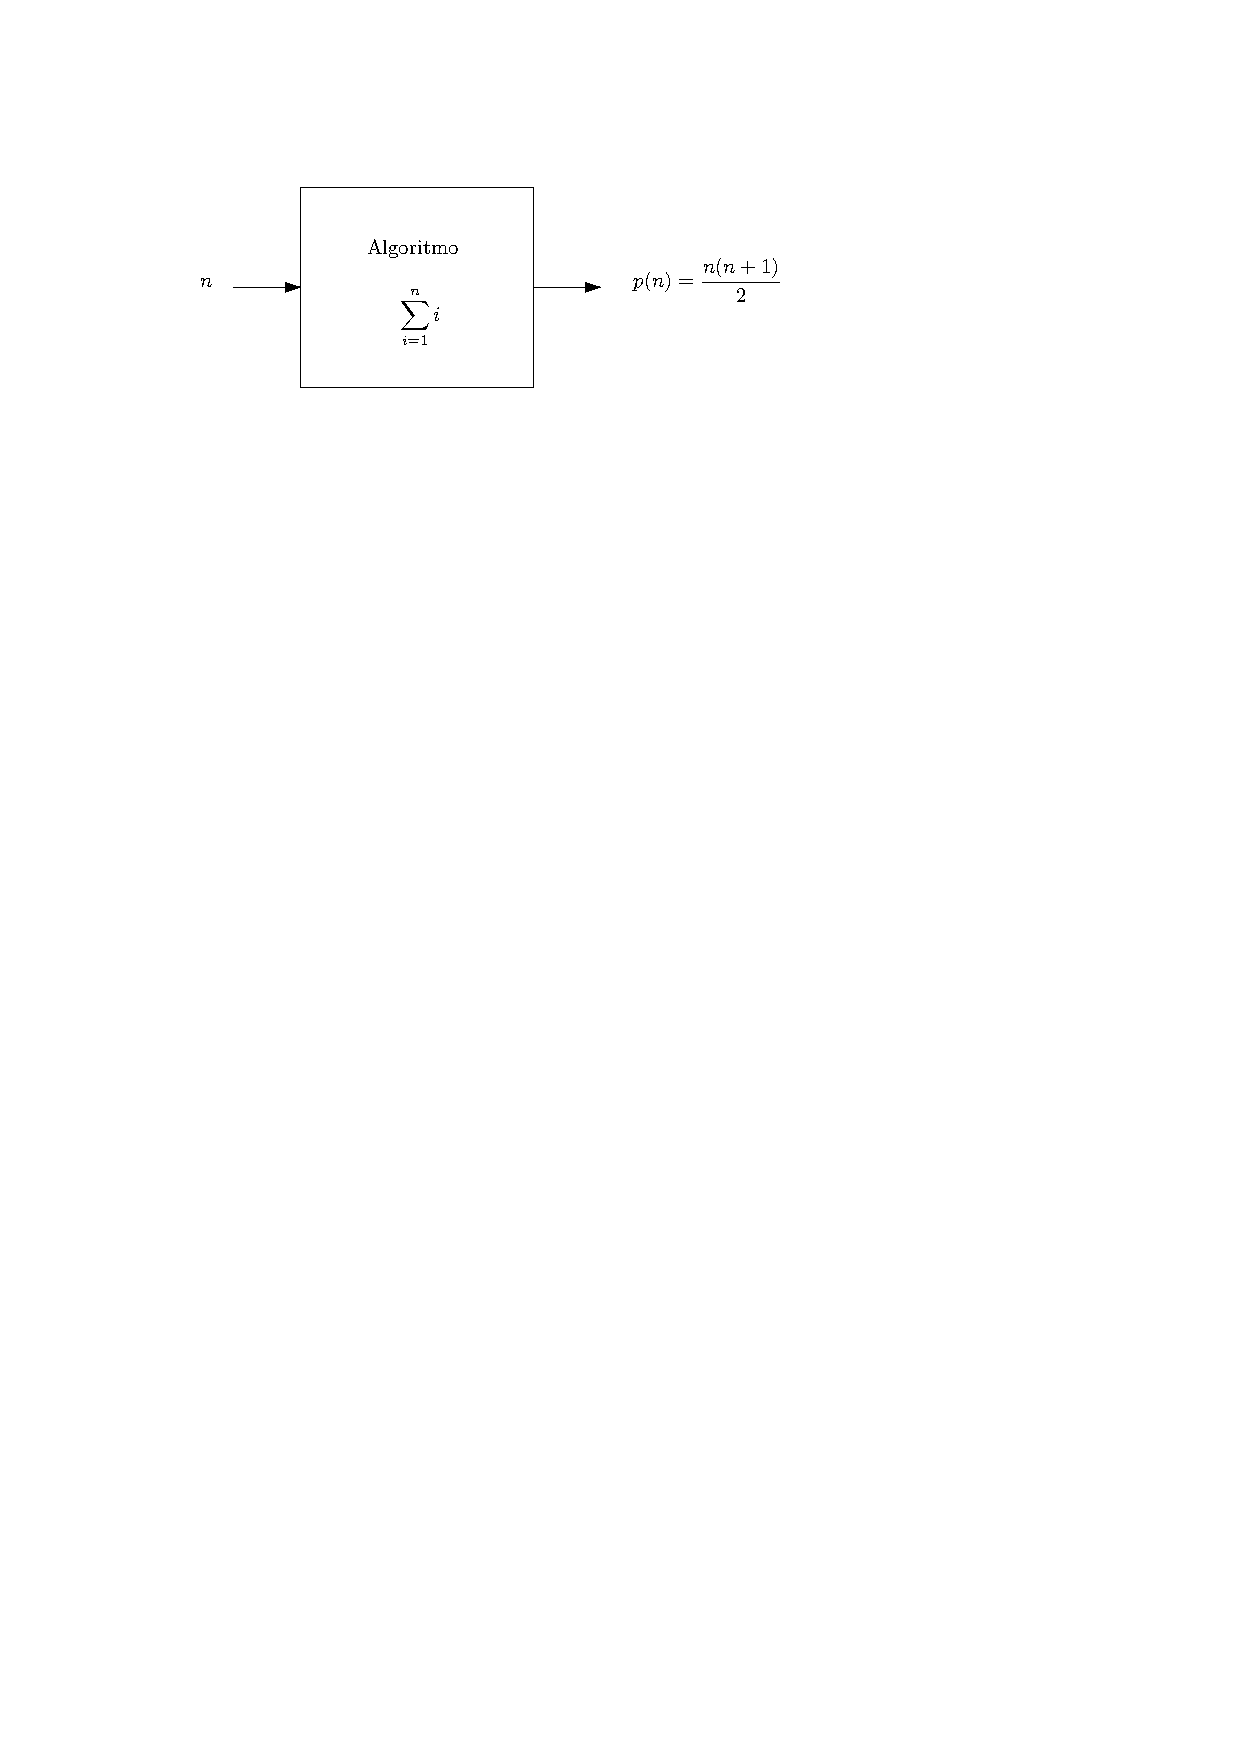
\includegraphics[width=14cm]{\figs/algoritmo} 
\end{figure}
\begin{itemize}
    \item No tenemos pruebas, pero tampoco dudas. (Elmo).
\end{itemize}
\begin{figure}[H]
    \centering
    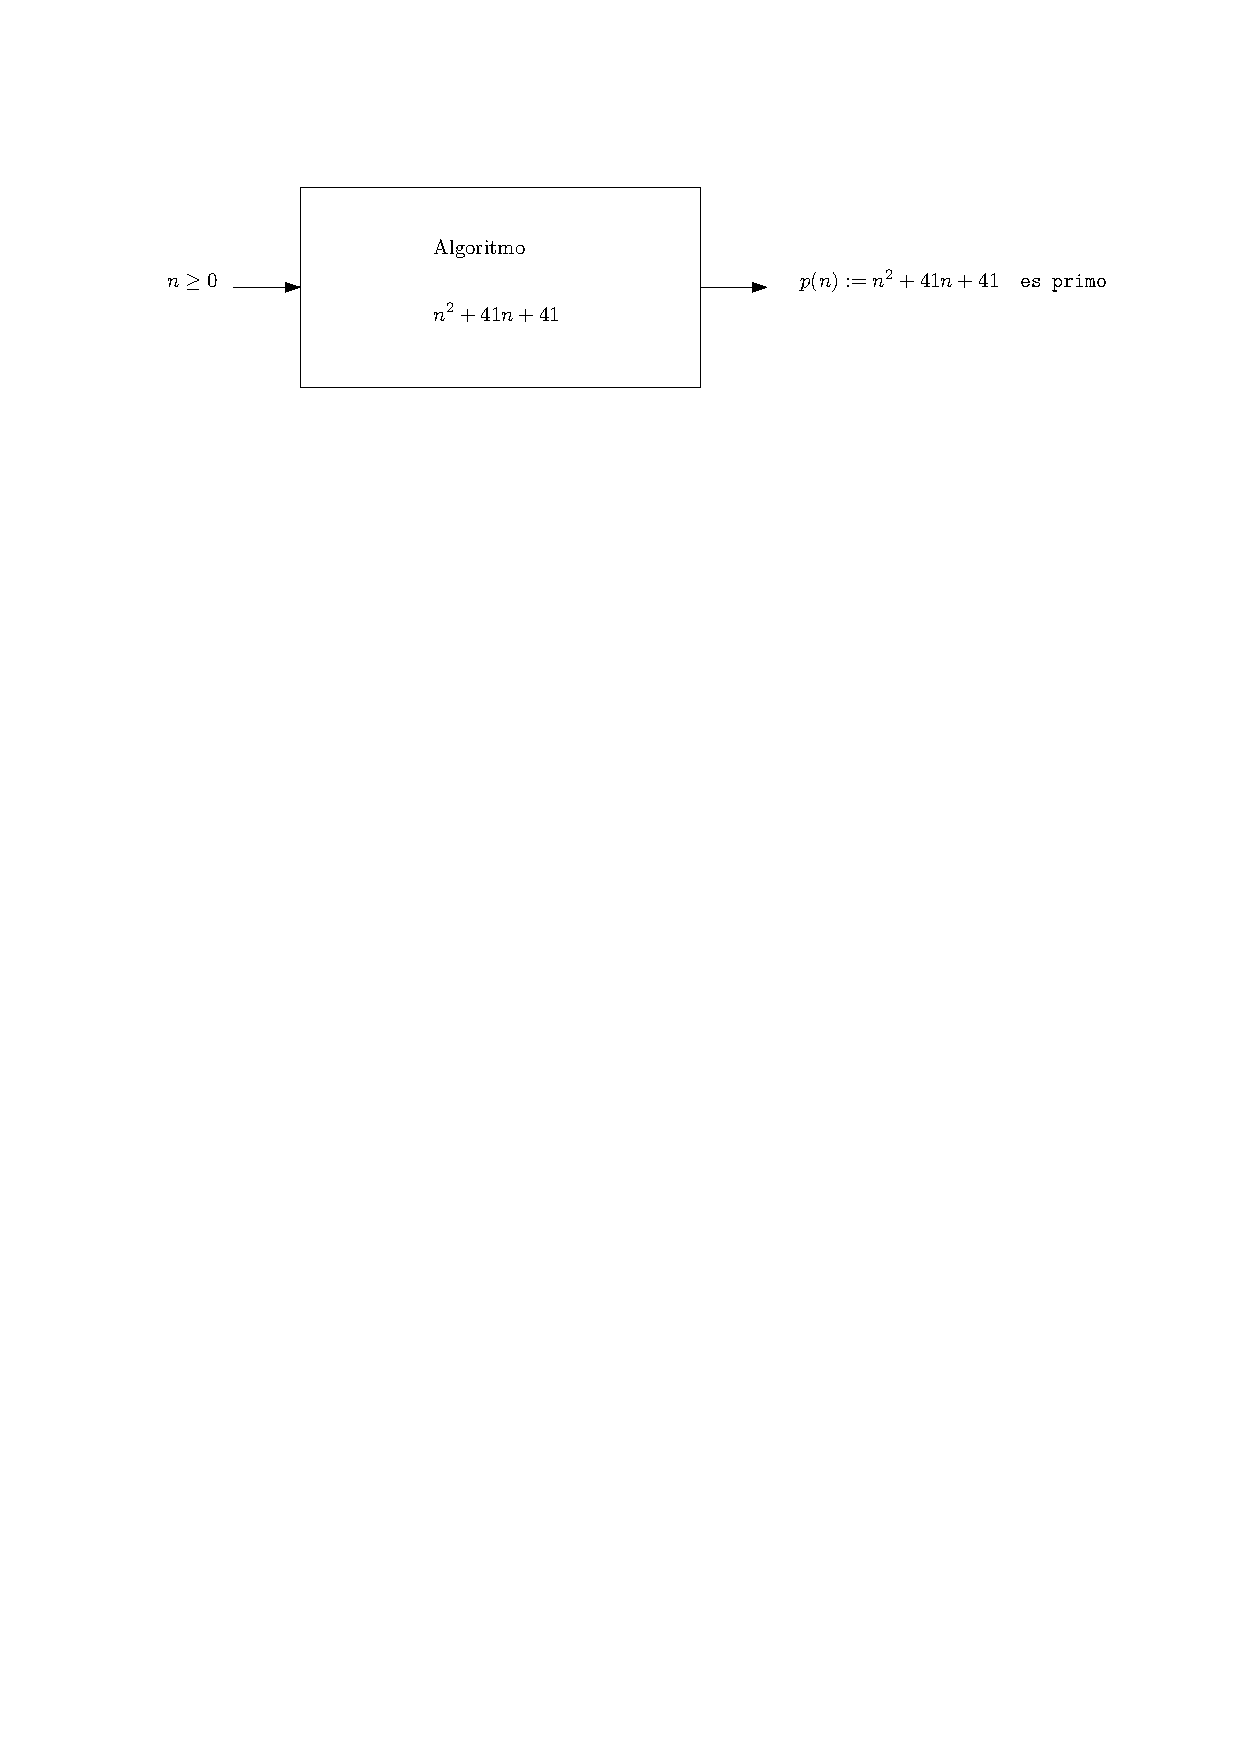
\includegraphics[width=14cm]{\figs/algoritmofalse} 
\end{figure}
